\documentclass[
  paper=a4,
  fontsize=12pt,
  DIV=16,
  headheight=30pt,
  footheight=45pt,
  headinclude,
  parskip=half,
]{scrartcl}

\usepackage{fontspec}
\setsansfont{Source Sans Pro}
\renewcommand{\familydefault}{\sfdefault}
\newfontfamily\geomfont{DejaVu Sans}
\newcommand\checkbox{{\geomfont\symbol{"25A2}}}

\usepackage{polyglossia}
\setmainlanguage{german}

\usepackage{microtype}
\usepackage{graphicx}
\usepackage[table]{xcolor}

\usepackage{scrlayer-scrpage}
\pagestyle{scrheadings}
\setkomafont{pagehead}{\normalfont}
\setkomafont{pagefoot}{\normalfont\footnotesize}
\ohead{
\includegraphics[height=1.5cm]{images/logo-pfeil-gruen.pdf}}
\ihead{%
  \large\textbf{Infobrief zur PhysiKon 2022}\\%
}
\cfoot{%
  \parbox[c]{0.3\textwidth}{%
    PEP et al.\ e.\,V.\\
z.\,Hd.\ Marie Schmitz\\
Otto-Hahn-Straße 4a\\
44227 Dortmund%
%
  }%
}

\ofoot{%
  \parbox[c]{0.3\textwidth}{%
%   Bankverbindung\\
  PeP et al.\\
Dortmunder Volksbank\\
IBAN:\@ \mbox{DE22 4416 0014 6348 4161 00}\\
BIC:\@ GENODEM1DOR%%
  }%
}
\ifoot{%
  
\includegraphics[height=1cm]{pep.pdf}\\
  \url{www.pep-dortmund.org}
}


\usepackage{titling}
\usepackage{booktabs}
\usepackage{enumitem}
\usepackage{csquotes}

% \usepackage{xcolor}
\usepackage{calc}
\usepackage[colorlinks=true,urlcolor=blue!50!black]{hyperref}
\renewcommand{\arraystretch}{1.5}

\newcommand\MyTextField[2][]{\TextField[#1, backgroundcolor=black!10, charsize=0pt, borderwidth=0]{#2}}
\renewcommand*{\LayoutTextField}[2]{\makebox[\widthof{#1: }][l]{#1: }%
\raisebox{0.8\baselineskip}{\raisebox{-\height}{#2}}}


\begin{document}

\textbf{\Large Herzlich Willkommen zur PhysiKon-Woche 2022!}

\vspace{1cm}
Schön, dass Sie bei unserer Jobmesse PhysiKon mit an Board sind!
In diesem Jahr wird die Jobmesse in einem hybriden Format vom 25. bis 28.04.2022 stattfinden.
Im folgenden Schreiben können wir hoffentlich alle wichtigen Fragen zur Veranstaltung beantworten.
Falls noch Fragen offen sind, melden Sie sich gerne bei uns!

\section*{Kontakt}

Sie erreichen das gesamte Team für organisatorische Rückfragen per Mail unter \href{mailto:physikon@pep-dortmund.org}{physikon@pep-dortmund.org}.
In dringenden Fällen und während des Messetags erreichen Sie uns telefonisch unter
\begin{itemize}
  \item Stefan Grisard: 0157 3265 4666
  \item Lena Linhoff: 0172 9726 790
  \item Thomas Honermann: 0151 6120 4192
  \item Jan-Peter Herdieckerhoff: 0157 8239 0765
\end{itemize}

\section*{Online-Vorträge}
\subsection*{Technische Voraussetzungen}

Die Online-Vorträge der PhysiKon 2022 werden über das Videokonferenzsystem \textbf{Zoom} stattfinden.
Sie benötigen dafür eine stabile Internetverbindung, einen Internetbrowser (am besten Safari oder Firefox), einen Lautsprecher und Mikrofon oder ein Headset.
Das Zoom-Meeting wird von uns organisiert und ist nur nach einer Registrierung zugänglich.

\subsection*{Zoom-Link}
Bitte registrieren Sie sich unter folgendem Link für die Online-Vorträge:

\url{https://tu-dortmund.zoom.us/meeting/register/tJcrduyrqjsvGNY2hORq-oBAoQMhVFmooIjU}

Falls Sie sich mit der Software nicht auskennen und eine Generalprobe durchführen möchten, geben Sie uns einfach Bescheid.
Wir organisieren gerne ein kurzes Test-Meeting mit Ihnen!

\subsection*{Breakout Rooms}
Zoom stellt eine \enquote{Breakout-Room}-Funktion zur Verfügung.
So können sich kleinere Gruppen in separaten Räumen unterhalten.
Wir werden diese Funktion anbieten, damit Sie sich zum Beispiel nach Ihrem Vortrag noch mit interessierten BesucherInnen weiter austauschen können, wenn der nächste Vortrag schon startet.
Denkbar wäre auch, dass Sie sich nach einer allgemeinen Vorstellung mit mehreren VertreterInnen Ihres Unternehmens (vielleicht aus verschiedenen Fachbereichen) auf verschiedene Zoom-Räume verteilen.
Dies sei nur als Anregung erwähnt, Sie müssen die Breakout-Funktion selbstverständlich nicht nutzen.

\subsection*{Moderation}
Die Moderation wird von uns übernommen, sodass Sie sich voll auf Ihren Vortrag konzentrieren können.
Zoom hat eine Chat-Funktion, die die Teilnehmenden nutzen können, um Fragen zu stellen.
Grundsätzlich ist es aber auch für Teilnehmende möglich, Mikrofon und Kamera einzuschalten und die Fragen direkt zu stellen.
Erfahrungsgemäß ist es am einfachsten, wenn die Moderation die Fragen sammelt und im Anschluss an Ihren Vortrag sortiert an Sie weiter gibt.
Falls Sie diesen Modus ändern möchten, geben Sie uns einfach Bescheid.


\subsection*{Technik-Check}
Sie haben die Möglichkeit vor Ihrem Vortrag Bild und Ton zu überprüfen.
Dazu können Sie entweder jeden Tag zwischen 12:30 Uhr und 13:00 Uhr dem Zoom-Meeting beitreten, oder direkt vor Ihrem Vortrag in den Breakout-Room \enquote{Technik-Check} kommen.
Dort wird jemand erreichbar sein, der Ihnen bei eventuellen Problemen helfen kann.


\subsection*{Ablauf und Präsentation}
Sie haben eine Stunde zur Verfügung, die Sie im Grunde frei gestalten können.
Klassischerweise können Sie einen Vortrag halten und Ihre Folien über das Videokonferenzsystem mit den Publikum teilen.
Der Vortrag sollte ungefähr 20 Minuten lang sein, damit genug Zeit für Fragen und den Austausch mit den Studierenden bleibt.
Wenn Sie kreative Ideen haben, wie Sie die Stunde interaktiver nutzen können, bringen Sie diese gerne mit ein!
Wir helfen gerne bei der Umsetzung.

Inhaltlich könnte Ihre Präsentation folgende Punkte abdecken:
\begin{itemize}
    \item Allgemeine Vorstellung des Unternehmens (Standort, Branche, Größe, Aufgabenfelder)
    \item Arbeitsfelder für MINT-Fachkräfte
    \item Einstiegsmöglichkeiten
    \item Falls vorhanden: Typischer Arbeitsalltag, Gehaltsstruktur
    \item Gerne: Persönlicher Werdegang, Einblick in Ihre persönliche (MINT-)Tätigkeit beim Unternehmen
\end{itemize} 

Diese Liste ist nicht vollständig und als Anregung gedacht.
Sie können Ihren Vortrag natürlich beliebig gestalten.

\subsection*{Zeiteinteilung Online-Vorträge}

\begin{table}[h!]
    \centering
\begin{tabular}{|c|l|}
    \hline
    \multicolumn{2}{|c|}{Montag, 25.04.2022} \\
    \hline
    \rowcolor{gray!10} 13 - 14 Uhr &  \\
    \rowcolor{gray!30} 14 - 15 Uhr & CGI \\
    \rowcolor{gray!10} 15 ­- 16 Uhr & RTL \\
    \rowcolor{gray!30} 16 - 17 Uhr & Amprion\\
    \rowcolor{gray!10} 17 ­- 18 Uhr & Elmos \\
    \hline
    \multicolumn{2}{|c|}{Dienstag, 26.04.2022} \\
    \hline
    \rowcolor{gray!10} 13 - 14 Uhr & Cohausz \& Florack \\
    \rowcolor{gray!30} 14 - 15 Uhr & Point 8 \\
    \rowcolor{gray!10} 15 ­- 16 Uhr & Ritzenhoefer \& Company \\
    \rowcolor{gray!30} 16 - 17 Uhr & Infineon \\
    \rowcolor{gray!10} 17 ­- 18 Uhr & zeb \\
    \hline
    \multicolumn{2}{|c|}{Mittwoch, 27.04.2022} \\
    \hline
    \rowcolor{gray!10} 13 - 14 Uhr & Ministerium für Schule \& Bildung NRW \\
    \rowcolor{gray!30} 14 - 15 Uhr & Deichmann \\
    \rowcolor{gray!10} 15 ­- 16 Uhr & Forschungszentrum Jülich \\
    \rowcolor{gray!30} 16 - 17 Uhr & NRW.BANK\\
    \rowcolor{gray!10} 17 ­- 18 Uhr & TNG Consulting \\
    \hline
    \end{tabular}

\end{table}


\section*{Messetag am 28. April 2022}

\subsection*{Ausstellernamensschilder}

\textbf{Bitte teilen Sie uns bis zum 07.04.2022 die Anzahl und Namen des Standpersonals mit}, damit wir vorab die passenden Namensschilder gestalten können.
Falls Sie in Ihrem Team Corona-bedingte Ausfälle fürchten, können Sie auch gerne mehr Namen einreichen, dann machen wir die Namensschilder für die eventuelle Vertretung schon mit fertig.

\subsection*{Adresse}

Technische Universität Dortmund\\
Emil-Figge-Straße 50\\
44227 Dortmund

\subsection*{Anfahrt}

Wenn Sie mit der Bahn anreisen, erreichen Sie den Campus der TU vom Dortmunder Hauptbahnhof aus mit der S1 Richtung Solingen.
Der Veranstaltungsort befindet sich in direkter Nähe zur S-Bahn-Station \enquote{Dortmund Universität}.

Wenn Sie mit dem Auto anreisen, stehen Ihnen Parkmöglichkeiten auf dem Parkplatz unter der Mensabrücke am Vogelpothsweg oder an der Emil-Figge-Straße (Einfahrt 18) zur Verfügung.
Sollten Sie mit schwerem Gepäck anreisen, können Sie mit dem Auto zum Ausladen bis vor das Gebäude der Emil-Figge-Straße 50 fahren.
Dazu fahren Sie von der Emil-Figge-Straße aus in die Einfahrt 19 und halten sich rechts.
Dann fahren Sie weiter geradeaus, bis Sie zur Polleranlage kommen.
Dort können Sie über die Ruftaste direkt mit der Leitwarte sprechen.
Geben Sie dort Bescheid, dass Sie zum Abladen für eine Veranstaltung in der EF50 vorfahren wollen und dann wird die Leitwarte die Poller absenken.
Unmittelbar nach dem Abladen müssen Sie Ihr Fahrzeug dann auf einem der umliegenden Parkplätze abstellen.
Direkt vor dem Gebäude gibt es keine Parkplätze.

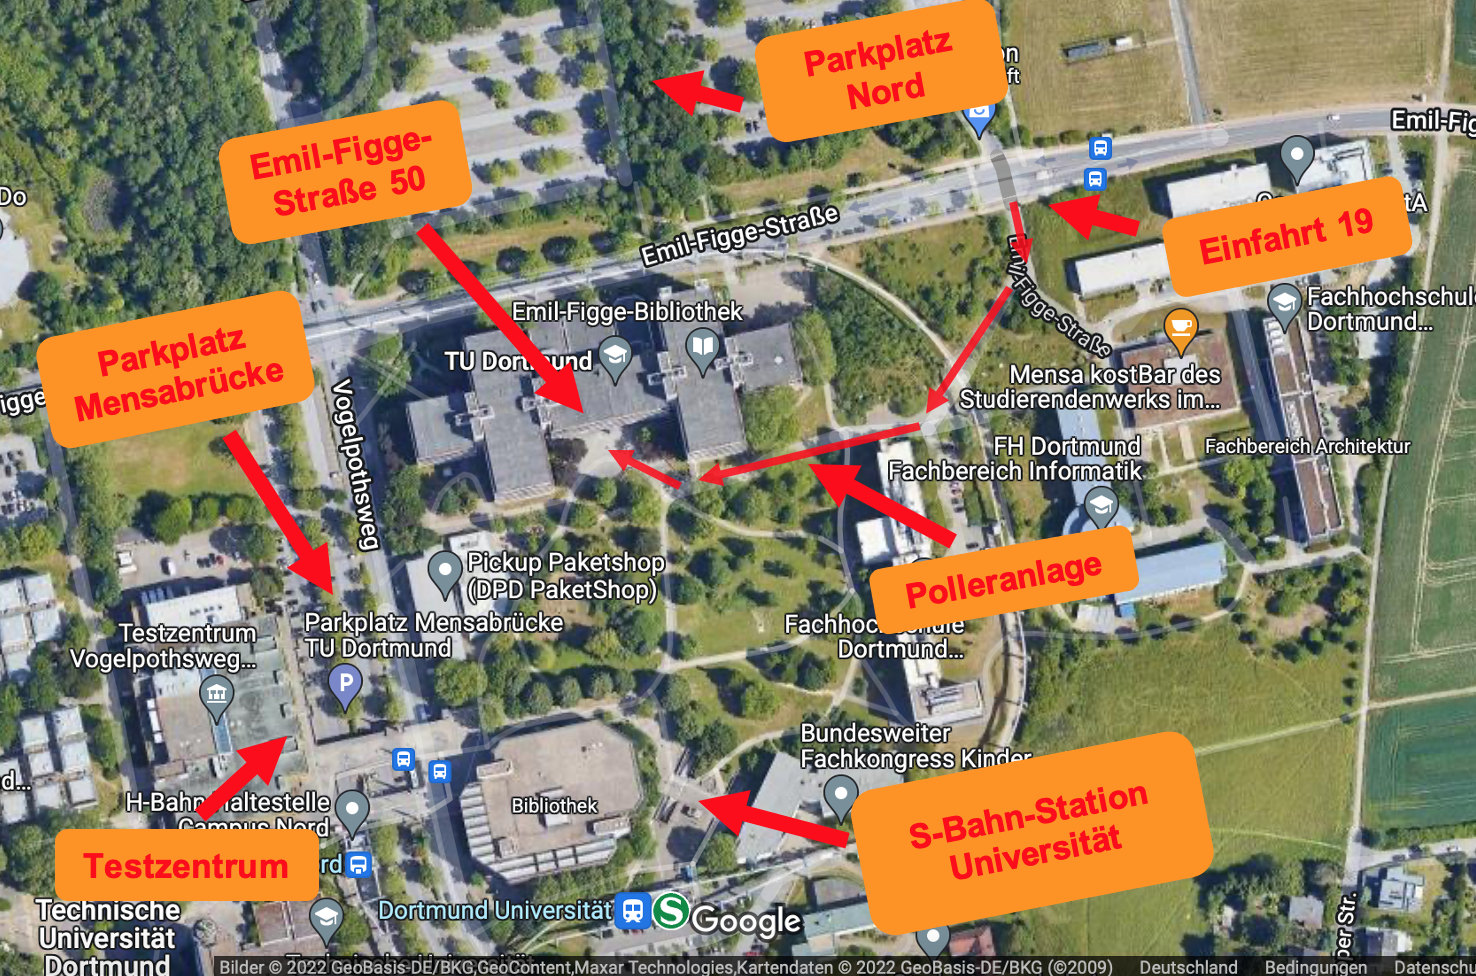
\includegraphics[width=\textwidth]{images/anfahrtskizze.jpg}


\subsection*{Ablaufplan}
\begin{description}
    \item[\textbf{08:00-10:00}] Aufbau\\
      Ab 8 Uhr können Sie anreisen und Ihren Messestand im Foyer der Emil-Figge-Straße 50 aufbauen.
      Vor Ort werden Helfer sein, die Ihre Fragen beantworten und Sie bestmöglich unterstützen.
      Stehtische, Tische und Stromanschlüsse finden Sie ebenfalls vor Ort.
    \item[\textbf{10:00-16:00}] Messe\\
      Die PhysiKon findet zwischen 10 und 16 Uhr statt.
      Während der gesamten Veranstaltung können Sie sich in unserem Aussteller-Bistro mit Speisen und Getränken versorgen.
    \item[\textbf{16:00-17:00}] Abbau\\
      Ab 16 Uhr können Sie mit dem Abbau Ihres Stands beginnen.
  \end{description}

\subsection*{Standplan}

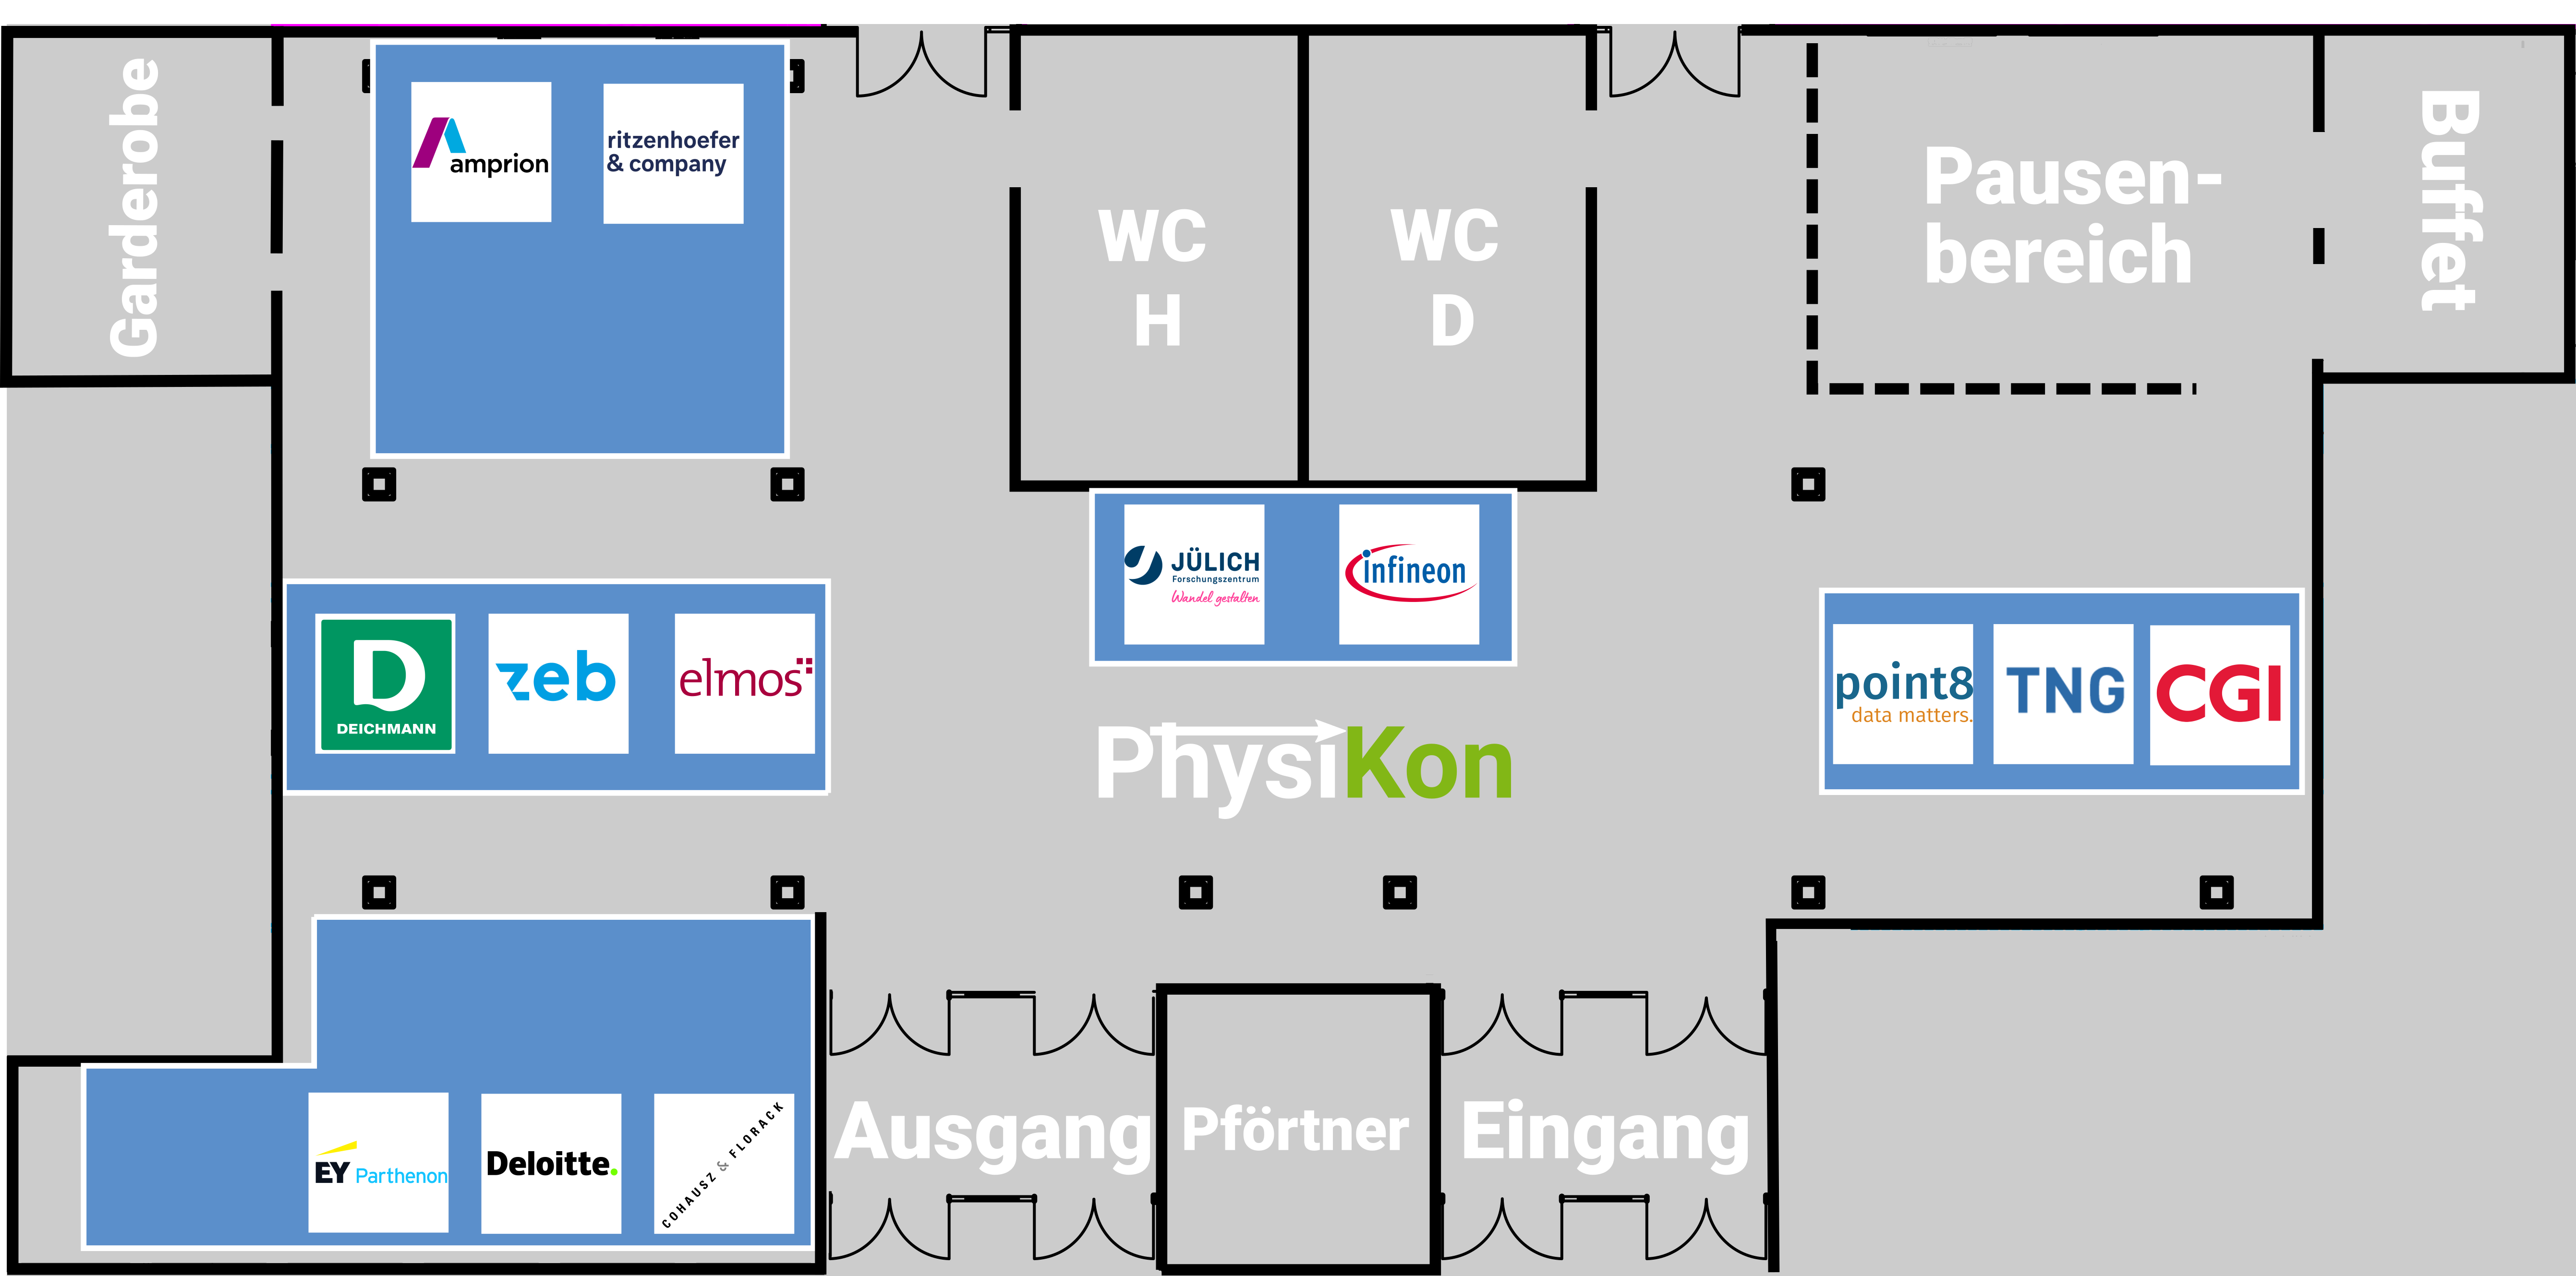
\includegraphics[width=\textwidth]{images/messeplan.png}


\subsection*{Standgestaltung}
Ihre Standfläche ist 2,5\,m$\times$2,5\,m groß.
Wir bitten darum, keine Aufbauten mitzubringen, die größer sind!
Roll-Up-Banner, Prospektständer etc. können gerne aufgestellt werden.

Die Stände können mit Strom versorgt werden, allerdings haben wir keinen Starkstrom zur Verfügung.
Bitte bringen Sie keine riesigen Beleuchtungsanlagen oder LED-Wände mit.
Strom für kleinere Bildschirme oder Laptops wird vorhanden sein.
Die Steckdosen sind teilweise unter der Decke.
Wenn Sie ein Verlängerungskabel griffbereit haben, können Sie dies gerne mitbringen.
Wir werden aber auch Verlängerungskabel vor Ort haben.

Tische und Stehtische werden von uns zur Verfügung gestellt.


\subsection*{Catering}
Für Ihr leibliches Wohl wird während der gesamten Veranstaltung gesorgt sein.
Das Catering wird vom Studierendenwerk serviert.
Vor dem Beginn der Messe starten wir mit einem kleinen Frühstück, außerdem wird es eine warme Mahlzeit zu Mittag und im Anschluss Kuchen geben.
Getränke werden ebenfalls vorhanden sein.


\subsection*{Hygienekonzept}
Soweit nicht anders angekündigt, gilt im Gebäude eine Maskenpflicht.
Wenn Sie eine Maske tragen, müssen Sie keinen Mindestabstand zu anderen Menschen einhalten.
Da Sie zum Essen Ihre Maske abnehmen müssen, gilt im Catering-Bereich ein Mindestabstand von 1,5\,m!
Wir werden die Sitzplätze dort so positionieren, dass dieser Abstand eingehalten werden kann.
Sollte es das Wetter zulassen, besteht auch die Möglichkeit, die Pause nach draußen zu verlegen.
Dort muss dann kein Mindestabstand eingehalten werden.

Sehr wahrscheinlich wird am Messetag (28.04.2022) die 3G-Regelung für alle Gebäude der TU Dortmund entfallen.
Das heißt, dass Sie das Gebäude ohne Impf- oder Testnachweis betreten können und auch die Besucher keinen 3G-Nachweis vorzeigen müssen.
Sollte sich die Corona-Lage bis zum Messetag noch mal verschlimmern, ist die wahrscheinlichste Konsequenz, dass Sie einen Impf- oder Testnachweis beim Betreten des Gebäudes vorzeigen müssen.

Wir legen allen Ausstellern und Besuchern der Messe wärmstens ans Herz vor der Veranstaltung einen Coronatest zu machen.
Ein Schnelltestzentrum gibt es zum Beispiel direkt am Parkplatz unter der Mensabrücke (Teststelle Vogelpothsweg \url{https://covidtest-dortmund.de/}) oder am REFA Center (\url{https://top-tagung.de/coronaschnelltestzentrumdortmund}).


\section*{Ausstellergebühr}
Die Teilnahme an der Präsenzmesse kostet 1000 Euro, für die ausschließliche Teilnahme an den Online-Vorträge berechnen wir 750 Euro.
Sie erhalten die Rechnung über die Ausstellergebühr Anfang Mai.
\textbf{Bitte teilen Sie uns hierfür noch die korrekte Rechnungsadresse mit}, falls noch nicht geschehen.\\
PeP et al. e.\,V. unterstützt als gemeinnütziger Verein die Fakultät Physik in Forschung und Lehre und fördert das Netzwerk der Studierenden und Alumni.
Durch den Ausstellerbeitrag unterstützen Sie unsere Projekte, die wir in ehrenamtlicher Arbeit für die Studierenden der Physik umsetzen.

\section*{Jobbörse}

Falls Sie aktuelle Stellenausschreibungen haben, veröffentlichen wir diese gerne in unserer PeP Jobbörse (\url{https://pep-dortmund.org/jobboerse}).
Die Jobbörse ist unabhängig von der PhysiKon immer über unsere Homepage erreichbar.
Senden Sie uns Ihre Stellenausschreibungen an \href{mailto:jobboerse@pep-dortmund.org}{jobboerse@pep-dortmund.org}

\vspace{0.5cm}

Sollten noch Fragen offen sein, geben Sie uns gerne Bescheid (Email: \href{mailto:physikon@pep-dortmund.org}{physikon@pep-dortmund.org}).
Wir freuen uns auf eine erfolgreiche PhysiKon 2022 mit Ihnen!

% \vspace{1cm}
Ihr PhysiKon-Team und PeP et al. e.\,V.

\end{document}